%% Normalidade Contextual em APIs -- versão 4 (14 recursos de alto volume, junho a setembro de 2026)
%% Classe acmart (sigconf), compatível com Overleaf (pdfLaTeX, XeLaTeX ou LuaLaTeX).
\documentclass[sigconf,nonacm]{acmart}

\usepackage[brazilian]{babel}
\usepackage{booktabs}
\usepackage{amsmath}
\usepackage{xspace}
\usepackage{fancyvrb}

\citestyle{acmauthoryear}
\settopmatter{printacmref=false, printfolios=true}
\renewcommand{\keywordsname}{Palavras-chave}
\setlength{\emergencystretch}{1.5em}

\newcommand{\Normal}{\textsc{Normal}\xspace}
\newcommand{\Residual}{\textsc{Residual}\xspace}

\begin{document}

\title{Normalidade Contextual em APIs: Caracterização de Regimes a partir de Access Logs para Apoio à Análise de Incidentes}

\author{Diego Paz Casagrande}
\affiliation{%
  \institution{Universidade de Brasília}
  \city{Brasília}
  \state{DF}
  \country{Brasil}}

\renewcommand{\shortauthors}{D. P. Casagrande}

\begin{abstract}
Quando um incidente é aberto, uma das primeiras perguntas do operador é se as APIs envolvidas estão operando normalmente e, se não estão, qual indicador saiu do padrão. A resposta não é trivial, porque o comportamento de uma API varia legitimamente com o horário, o calendário e os processamentos em lote, e muda ao longo dos meses. Este trabalho investiga se \emph{API Access Logs} (AALs) agregados por minuto permitem responder, no instante do registro do incidente, se cada recurso de API está em um de seus regimes normais (\Normal) ou fora deles (\Residual); qual indicador é responsável: erros de negócio (4xx), erros de sistema (5xx) ou latência; e desde quando. Seguindo o CRISP-DM, propõe-se um perfil de normalidade contextual por recurso (mediana e MAD por hora e tipo de dia), com um limite próprio para cada indicador calibrado por validação cruzada, e uma expansão retroativa em faixas de 15~min a 4~h para estimar o início do desvio. O estudo usa 14 recursos de produção com dados completos de junho a setembro de 2026 (24,5 milhões de registros e 3,5 bilhões de transações): o perfil é ajustado com junho a agosto e testado em 8.891 consultas simuladas em setembro. A decisão sobre os 15 minutos anteriores ao registro teve especificidade de 97,3\%, sensibilidade de 63\% (71\% nas degradações de intensidade média e alta), indicador correto em 98,2\% dos casos detectados e início dentro da zona estimada em 94,8\% deles. Erros de sistema foram detectados em até 99\% dos casos e a latência em 90\% nas degradações de 10 vezes. Um histórico de 1 mês superou o de 3 meses, o que indica que o retreino frequente é preferível a um histórico longo.
\end{abstract}

\keywords{Mineração de Dados; API Access Log; Normalidade Contextual; Análise de Incidentes; CRISP-DM; Regimes Operacionais.}

\maketitle

%% =====================================================================
\section{Introdução}

A arquitetura dos sistemas modernos consolidou o uso de APIs (\emph{Application Programming Interfaces}) como mecanismo fundamental de integração em sistemas distribuídos. Em ambientes corporativos de grande porte, as APIs medeiam desde requisições de clientes externos até transações entre sistemas legados e modernos. No Banco do Brasil, cerca de 30 mil APIs são executadas diariamente, conectando soluções de negócio que combinam plataformas em nuvem e \emph{mainframe}.

\subsection{Contexto}
Requisições processadas por gateways de API geram registros com o instante da execução, o recurso acessado, o código de resposta, o tempo de processamento e o consumidor. Neste estudo, esses registros são denominados \emph{API Access Logs} (AALs): o registro gerado pelo gateway para as requisições processadas, distinto do \emph{execution log} e do log de aplicação. Os AALs estão disponíveis de forma padronizada para um conjunto amplo de APIs, sem instrumentação específica no código.

O comportamento de uma API não é estacionário. Volume, latência e proporção de erros variam com o horário, o dia da semana, os processamentos em lote e as janelas de manutenção, e também mudam de patamar ao longo dos meses. Uma taxa de erros que é normal na virada do dia, durante um lote, pode ser anormal às 10h de um dia útil.

\subsection{Problema}
Quando um incidente é registrado, o operador precisa responder, para cada API envolvida: \emph{no momento em que o incidente foi aberto, a API está operando dentro de um regime normal?} Se não está, importa saber \emph{qual indicador foi impactado}: erros de negócio (faixa 4xx), erros de sistema (faixa 5xx) ou latência; e \emph{desde quando} o desvio acontece. Como informação complementar, interessa saber se o impacto é \emph{generalizado} ou concentrado em um \emph{consumidor específico}, com volume suficiente para alterar o resultado agregado da API.

Hoje essa resposta depende de consultar várias ferramentas e de conhecer o comportamento típico de cada API~\citep{zhang2025isre}. Limites fixos ou um único perfil de normalidade não distinguem a variação legítima (um lote à meia-noite, o volume menor no fim de semana) de um desvio real.

Do ponto de vista de mineração de dados, o problema consiste em: (1) caracterizar os regimes normais de cada recurso a partir de AALs agregados; (2) classificar o período imediatamente anterior ao registro de um incidente em dois estados: \Normal (dentro de algum regime normal esperado para aquele contexto) ou \Residual (todo o resto); e (3) quando \Residual, identificar o indicador responsável e o início do desvio.

\subsection{Motivação}
Este trabalho complementa um projeto de mestrado sobre sistemas multiagente para apoio ao atendimento de incidentes. A literatura recente mostra agentes especializados em diferentes fontes de dados, coordenados para triagem e análise~\citep{yu2025triangle,luo2025opsagent,zhang2025isre}. Um desses agentes precisa de uma fonte confiável e explicável sobre o comportamento das APIs. O foco não é monitoração em tempo real nem a identificação da causa raiz, mas a \emph{informação de contexto no instante do incidente}: dizer se cada recurso está em regime normal e, se não, qual indicador está impactado e desde quando. Essa informação abastece o operador e colabora para a análise do ocorrido.

\subsection{Objetivos}
\textbf{Objetivo geral:} caracterizar os regimes normais de cada recurso de API a partir de Access Logs agregados e, no instante do registro de um incidente, informar se o recurso está em regime normal e, se não, qual indicador foi impactado e desde quando.

\textbf{Objetivos específicos:}
\begin{itemize}
  \item Verificar se cada recurso apresenta vários regimes normais ligados ao contexto (hora e tipo de dia).
  \item Construir um perfil de normalidade por recurso e contexto e uma regra de decisão \Normal/\Residual explicável.
  \item Identificar o indicador responsável (4xx, 5xx, latência) e estimar o início do desvio.
  \item Avaliar o método em cenários de incidente simulados e compará-lo a baselines simples.
  \item Avaliar quanto histórico o perfil precisa (3 meses ou 1 mês).
  \item Disponibilizar a informação em formato estruturado para um agente ou operador.
\end{itemize}

\subsection{Questões de pesquisa}
\begin{itemize}
  \item \textbf{RQ1.} AALs agregados permitem caracterizar os regimes normais de cada recurso e decidir, no instante do registro, se o recurso está em regime normal?
  \item \textbf{RQ2.} Quando o recurso não está em regime normal, o método identifica corretamente o indicador responsável (4xx, 5xx, latência) e o início do desvio?
  \item \textbf{RQ3.} Qual o período anterior ao registro (15, 30 ou 60~min) mais adequado para a decisão, e como o intervalo entre o início da degradação e o registro afeta o resultado?
  \item \textbf{RQ4.} Um histórico mais longo (3 meses) produz um perfil melhor do que o histórico recente (1 mês)?
\end{itemize}

\subsection{Contribuições e organização}
As contribuições são: (i) a caracterização empírica dos regimes de 14 recursos de API de produção de alto volume; (ii) um método simples e explicável, sem rótulos, que decide o estado de um recurso no instante do registro e aponta o indicador impactado; (iii) uma estimativa de início por expansão retroativa; (iv) um protocolo de avaliação com cenários de incidente simulados; e (v) evidência de que o histórico recente é mais útil que o longo. A Seção~\ref{sec:correlatos} discute os trabalhos correlatos; a Seção~\ref{sec:metodologia}, a metodologia; a Seção~\ref{sec:resultados}, os resultados; a Seção~\ref{sec:discussao}, a discussão; a Seção~\ref{sec:ameacas}, as ameaças à validade; e a Seção~\ref{sec:conclusao} conclui.

%% =====================================================================
\section{Trabalhos correlatos}\label{sec:correlatos}

\subsection{Análise e mineração de logs}
\citet{du2017deeplog} propuseram o DeepLog, que emprega redes LSTM para aprender sequências normais de eventos de log e sinalizar desvios. \citet{meng2019loganomaly} propuseram o LogAnomaly, que combina informação semântica dos \emph{templates} com a detecção de anomalias sequenciais e quantitativas. Ambos mostram que logs carregam informação suficiente para caracterizar comportamento, mas operam sobre sequências de eventos de logs de sistema, e não sobre AALs agregados; tampouco tratam da coexistência de múltiplos regimes normais.

\subsection{Normalidade e séries temporais}
\citet{siffer2017dspot} propuseram o SPOT/DSPOT, que calibra limiares a partir da cauda da distribuição com Teoria de Valores Extremos e os adapta a séries não estacionárias, mas sem identificar os contextos que fazem o limiar variar. \citet{audibert2020usad} propuseram o USAD, baseado em autoencoders para séries multivariadas, centrado em escores de anomalia, e não na interpretação de regimes. \citet{wang2025crosssystem} discutem a dificuldade de generalizar modelos entre sistemas distintos, o que reforça a opção por perfis ajustados por recurso.

\subsection{Modelagem comportamental de microsserviços}
O DeepTraLog~\citep{zhang2022deeptralog} combina \emph{traces} e logs em grafos, e o GAMMA~\citep{somashekar2024gamma} localiza gargalos com redes neurais em grafos. Esses trabalhos pressupõem \emph{traces}, logs internos ou métricas de infraestrutura, que extrapolam o AAL isolado.

\subsection{Incidentes e sistemas multiagente}
O Triangle~\citep{yu2025triangle} usa múltiplos agentes na triagem de incidentes; o OpsAgent~\citep{luo2025opsagent} e o trabalho de \citet{zhang2025isre} coordenam agentes especializados para análise de incidentes. Esses sistemas dependem de fontes que resumam o estado dos componentes de forma confiável. O presente trabalho se posiciona como uma dessas fontes: transforma AALs em evidência explicável sobre o estado de cada recurso no momento do incidente.

\subsection{Síntese e lacuna}
Os trabalhos revisados tratam o comportamento, predominantemente, a partir de um único perfil de normalidade; dependem de fontes além do AAL; ou focam na causa raiz. Nenhum investiga, a partir exclusivamente do AAL, a caracterização de múltiplos regimes normais por recurso e o seu uso para informar, no instante de um incidente, o estado do recurso, o indicador impactado e o início do desvio.

%% =====================================================================
\section{Metodologia}\label{sec:metodologia}

O trabalho segue o CRISP-DM~\citep{wirth2000crispdm,chapman2000crispdm}. Cada fase foi implementada em um \emph{notebook} Jupyter com parâmetros explícitos e sementes fixas (Tabela~\ref{tab:fases}). A análise é sempre \emph{por recurso}. Optou-se por técnicas simples de explicar: seis no total, todas disponíveis em pandas, SciPy e scikit-learn~\citep{pedregosa2011sklearn}.

\begin{table}[t]
  \caption{Fases do CRISP-DM, notebooks e técnicas.}
  \label{tab:fases}
  \small
  \begin{tabular}{p{0.2\columnwidth}p{0.7\columnwidth}}
    \toprule
    Fase & Notebook: conteúdo (técnica) \\
    \midrule
    Negócio, Dados & 01: problema, critérios de sucesso, extração e seleção dos recursos, qualidade e evolução mensal \\
    Preparação & 02: consolidação, atributos por janela, p95 de latência \\
    Dados, Modelagem & 03: regimes (Kruskal-Wallis; k-means) \\
    Modelagem & 04: perfil contextual (mediana/MAD); limite por indicador (validação cruzada), por histórico \\
    Preparação & 05: cenários de incidente (injeção de falhas) \\
    Avaliação & 06: estado, indicador, início (expansão retroativa); histórico; IC de Wilson, McNemar \\
    Implantação & 07: consulta estruturada para o agente \\
    \bottomrule
  \end{tabular}
\end{table}

\subsection{Entendimento do negócio}
A decisão apoiada é: \emph{no instante do registro do incidente, o recurso está em regime normal? Se não, qual indicador foi impactado (erros 4xx, erros 5xx, latência) e desde quando?} A abrangência (consumidor específico ou generalizado) é informação complementar. Os critérios de sucesso foram definidos antes da modelagem (Tabela~\ref{tab:criterios}). Como não havia histórico de incidentes, a avaliação usa cenários simulados com falhas injetadas.

\subsection{Entendimento dos dados}
A base original tem 118 milhões de linhas de AALs de produção de 18 recursos (\texttt{CD\_RCS\_CAT}), de maio a setembro de 2026. \textbf{Cada linha é um agregado por minuto $\times$ recurso $\times$ código HTTP $\times$ cliente}: o total de execuções no minuto (\texttt{QT\_TTL\_TRAN}) e o tempo médio dessas execuções (\texttt{QT\_TMP\_MEDI\_EXEA}). Não há registros por requisição. O identificador de cliente foi anonimizado por SHA-256 com semente, sem payloads nem dados pessoais. Os horários, em UTC, foram convertidos para o horário de Brasília (UTC$-3$) antes de qualquer corte temporal.

\paragraph{Seleção dos recursos.} Foram mantidos apenas os recursos com dados em \emph{todos os dias} de 01/06 a 20/09 (horário de Brasília): 14 dos 18, identificados aqui por A01 a A14 em ordem decrescente de volume. Os quatro descartados, com 7 a 16 dias sem dados, somavam 21\% do volume do período.

O recorte tem 24.495.617 linhas, 3,5 bilhões de transações e 5.506 clientes, de 01/06/2026 a 20/09/2026 20h59. As respostas 2xx somam 94,1\% das transações; 4xx, 5,8\%; 5xx, 0,09\%. Há 375.697 linhas excedentes com a mesma chave (minuto, recurso, código, cliente), que concentram 7,5\% do volume. Os recursos são de alto volume: a mediana de transações por 15~min vai de 453 (A14) a 85.335 (A01). O A08 atende 5.390 clientes; o A12, apenas 4. Dois recursos (A05 e A06) têm dados em todos os dias, mas não em todos os minutos (72\% e 77\% dos minutos).

\paragraph{Evolução mensal.} O volume dos maiores recursos é estável entre junho e setembro, mas alguns mudam de patamar: o A13 cai de 272 mil para 53 mil transações por dia; a taxa de erros de negócio do A08 passa de 8\% (junho) para 45\% (setembro), e a do A07, de 8,5\% para 0,7\%. Essa mudança motiva a questão RQ4.

\subsection{Preparação dos dados}
As chaves repetidas foram consolidadas (soma do volume e média de latência ponderada). Os registros foram agregados em janelas de 1~h (37.586 janelas recurso $\times$ hora) e em períodos de 15 e 30~min. A decisão usa quatro indicadores (Tabela~\ref{tab:atributos}). O \emph{contexto} de cada período é o par (tipo de dia, hora), com tipo de dia \emph{útil} ou \emph{não útil} (sábado, domingo e feriados: 04/06 e 07/09).

\paragraph{Latência p95.} Como não há latência por requisição, o p95 é o percentil 95 das latências médias por minuto $\times$ cliente das respostas 2xx, ponderado pelo número de execuções. É um p95 \emph{das médias}, não das requisições, e tende a subestimar a cauda real; mas é consistente entre períodos e sensível a degradações que atingem só parte dos minutos ou dos consumidores. Na mediana, ele é 1,21 vez a latência média.

\begin{table}[t]
  \caption{Indicadores usados na decisão e direção desfavorável.}
  \label{tab:atributos}
  \small
  \begin{tabular}{p{0.2\columnwidth}p{0.52\columnwidth}p{0.16\columnwidth}}
    \toprule
    Indicador & Definição & Direção \\
    \midrule
    volume & $\log(1+$transações$)$, na escala horária & alta e queda \\
    erros 4xx & transações 4xx / total (erros de negócio) & alta \\
    erros 5xx & transações 5xx / total (erros de sistema) & alta \\
    latência p95 & $\log(1+$p95 das médias por minuto$\times$cliente$)$ & alta \\
    \bottomrule
  \end{tabular}
\end{table}

\subsection{Modelagem}

\paragraph{Regimes (descritivo).} O teste de Kruskal-Wallis~\citep{kruskal1952ranks}, com correção de Bonferroni~\citep{dunn1961multiple}, verifica se cada indicador muda entre as 24 horas dos dias úteis. Para cada recurso, o k-means~\citep{lloyd1982kmeans} agrupa as janelas de 1~h de junho a agosto usando apenas os indicadores padronizados e limitados aos percentis 1 e 99 do recurso, para que picos isolados não formem grupos próprios. O número de regimes, $k\in[2,8]$, é escolhido pelo coeficiente de silhouette~\citep{rousseeuw1987silhouette}. O contexto não entra no agrupamento; ele é usado depois, para nomear cada regime (nível de volume, tipo de dia e horas em que predomina). O k-means é descritivo: a decisão usa o perfil contextual.

\paragraph{Perfil de normalidade contextual.} Para o recurso $r$, o contexto $c$ e o indicador $a$, o perfil guarda a mediana $m_a(r,c)$ e a escala robusta~\citep{leys2013mad}
\begin{equation}
  s_a(r,c)=\max\{1{,}4826\cdot\mathrm{MAD}_a(r,c),\ \varepsilon_a\},
\end{equation}
calculadas nas janelas de 1~h do histórico, em que $\varepsilon_a$ é um piso que evita divisões por valores próximos de zero. Para um período $w$, o desvio de cada indicador, contado só na direção desfavorável, é
\begin{equation}
  z_a(w)=\frac{x_a(w)-m_a(r,c)}{s_a(r,c)},
\end{equation}
\begin{equation}
  d_a(w)=\begin{cases}|z_a(w)| & \text{volume,}\\ \max\{z_a(w),0\} & \text{demais indicadores.}\end{cases}
\end{equation}
Períodos de 15 e 30~min usam o mesmo perfil de 1~h: o volume é convertido para a escala horária, e as taxas e o p95 são usados diretamente.

\paragraph{Limite por indicador.} Os indicadores têm variabilidades muito diferentes; em alguns recursos a taxa de 4xx tem picos reais frequentes. Por isso, cada indicador tem um limite próprio no recurso, $L_{r,a}=\max\{3,\ Q_{0{,}99}(d_a)\}$: o percentil 99 dos seus desvios no histórico, calculados fora da amostra. O limite é recalculado para cada tamanho de período (15, 30 e 60~min), porque períodos curtos variam mais. O período é \Residual se algum indicador passa do seu limite ($d_a/L_{r,a}>1$); o \textbf{indicador responsável} é o que mais passou, em múltiplos do limite.

\paragraph{Histórico e calibração sem vazamento.} O teste é em 01 a 20/09. O perfil e os limites são ajustados só com dados anteriores, em dois históricos: \emph{3 meses} (principal; junho a agosto) e \emph{1 mês} (agosto). Os desvios fora da amostra vêm de validação cruzada com quatro blocos contíguos de tempo dentro do histórico: o perfil é ajustado em três blocos e avalia o restante. Com essa regra, cerca de 3\% dos períodos do histórico são \Residual.

\paragraph{Início estimado (expansão retroativa).} A partir do registro, o método avalia faixas disjuntas cada vez mais distantes: 0--15, 15--30, 30--60~min e, depois, de hora em hora até 4~h, cada uma com o limite do seu tamanho. A busca para na primeira faixa \Normal, e o início é estimado entre o começo da última faixa residual e o fim dessa faixa normal.

\paragraph{Abrangência (complementar).} Para erros 4xx ou 5xx, o desvio é atribuído a um \emph{consumidor específico} quando o cliente com mais erros concentra ao menos 80\% deles e essa fatia supera em pelo menos 20 pontos percentuais a sua fatia do volume; caso contrário, é \emph{generalizado}. Períodos com menos de três clientes ativos ficam indeterminados.

\subsection{Avaliação}

\paragraph{Cenários de incidente.} Cada cenário simula um incidente: uma degradação começa em $t_0$ e o incidente é registrado em $t=t_0+\Delta$, com atraso $\Delta\in\{15,30,60,120\}$~min. O instante de registro é sorteado entre 01/09 às 04h e 20/09 às 21h. As falhas (Tabela~\ref{tab:falhas}) são aplicadas nos registros por minuto $\times$ cliente e depois reagregadas, para que os indicadores e a abrangência reajam como numa falha real. Foram gerados 5 cenários por recurso $\times$ motivo $\times$ intensidade $\times$ atraso (4.480 incidentes) e 4.480 consultas de controle, em instantes sem falha injetada. Sessenta e nove incidentes caíram em intervalos sem nenhum tráfego no recurso (sobretudo nos recursos com minutos sem dados), onde a falha não se manifesta, e foram excluídos: restam 4.411 incidentes e 4.480 controles.

\begin{table}[t]
  \caption{Motivos injetados.}
  \label{tab:falhas}
  \small
  \begin{tabular}{p{0.26\columnwidth}p{0.64\columnwidth}}
    \toprule
    Motivo & Intensidade (baixa / média / alta / muito alta) \\
    \midrule
    4xx generalizado & 5\% / 15\% / 40\% das 2xx viram 400 \\
    4xx de 1 consumidor & 30\% / 60\% / 90\% das 2xx do consumidor viram 400 \\
    5xx generalizado & 5\% / 15\% / 40\% das 2xx viram 503 \\
    5xx de 1 consumidor & 30\% / 60\% / 90\% das 2xx do consumidor viram 503 \\
    Latência & tempo de execução $\times$1,5 / $\times$2,5 / $\times$4 / $\times$10 \\
    \bottomrule
  \end{tabular}
  \par\smallskip\footnotesize O consumidor afetado é sorteado com probabilidade proporcional ao seu volume.
\end{table}

\paragraph{Latência $\times$10.} Como a latência vem de médias por minuto, poucas requisições lentas elevam muito o valor. No histórico, o p95 horário ultrapassou 10 vezes a mediana do seu contexto em 0,13\% das horas (percentil 99,9: 15 vezes; máximo: 59 vezes). Degradações de latência relevantes para um incidente podem ser desse tamanho, por isso a intensidade ``muito alta'' ($\times$10) foi incluída. As intensidades menores foram mantidas para mostrar o limite do método.

\paragraph{Métricas.} Para cada cenário, avalia-se o período $[t-L,t)$, com $L=15$~min como principal e 30 e 60~min para comparação. As métricas são: \emph{sensibilidade} (incidentes com saída \Residual); \emph{especificidade} (controles com saída \Normal); \emph{acurácia do indicador} (indicador apontado igual ao do motivo injetado, entre os detectados); \emph{acerto do início} (início real dentro da zona estimada); e \emph{acurácia da abrangência}. ``Média/alta'' refere-se às intensidades média e alta, sem a latência $\times$10. As proporções têm intervalos de confiança de Wilson a 95\%~\citep{wilson1927probable}.

\paragraph{Baselines.} Com o mesmo tratamento de limites e calibração: (i) \emph{z-score global}, o mesmo perfil sem contexto (um por recurso); e (ii) \emph{semana anterior}, que compara com o mesmo período sete dias antes. A comparação usa o teste exato de McNemar~\citep{mcnemar1947note} sobre os acertos de estado nos mesmos cenários; o mesmo teste compara os históricos de 3 meses e de 1 mês.

%% =====================================================================
\section{Resultados}\label{sec:resultados}

\subsection{Regimes normais por recurso (RQ1)}

A Figura~\ref{fig:perfis} mostra os quatro recursos com padrão horário mais marcado: lotes na madrugada (A05 às 2--3h; A09 à 0--1h e às 11h), lote na virada do dia e às 18h dos dias úteis (A10) e padrão comercial com menor volume em dias não úteis (A12). A Figura~\ref{fig:mapa} mostra que cada recurso tem sua própria assinatura horária de volume e de latência. Nos dias úteis, 93\% dos testes de Kruskal-Wallis (recurso $\times$ indicador) foram significativos após Bonferroni. O efeito mediano ($\varepsilon^2$) foi grande para volume (0,56), latência p95 (0,43), erros 4xx (0,25) e erros 5xx (0,21). A exceção é o A13, que só tem um indicador com variação horária significativa.

\begin{figure*}[t]
  \centering
  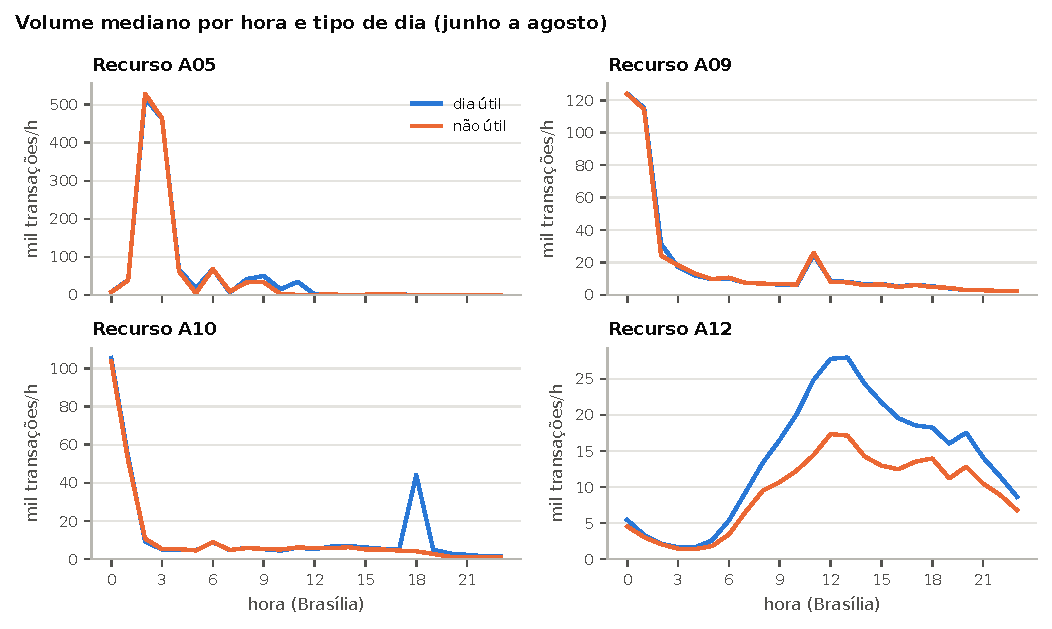
\includegraphics[width=0.9\textwidth]{figuras/fig_perfis_volume.pdf}
  \caption{Volume mediano por hora e tipo de dia (junho a agosto), nos quatro recursos com padrão horário mais marcado.}
  \label{fig:perfis}
\end{figure*}

\begin{figure*}[t]
  \centering
  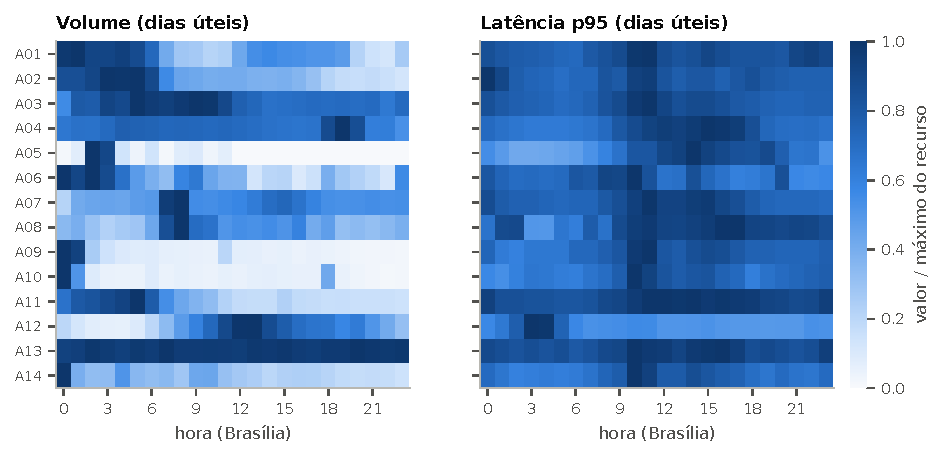
\includegraphics[width=0.85\textwidth]{figuras/fig_mapa_calor.pdf}
  \caption{Volume e latência p95 medianos por hora em dias úteis, normalizados pelo máximo de cada recurso.}
  \label{fig:mapa}
\end{figure*}

O k-means encontrou de 2 a 6 regimes por recurso (mediana 3; silhouette médio 0,54; Tabela~\ref{tab:recursos}). A Figura~\ref{fig:regimes} ilustra o A11: um regime de volume alto na madrugada (0--8h nos dias úteis, 0--6h nos não úteis) e um de volume baixo no restante do dia. É o tipo de variação legítima que um limite fixo trataria como anomalia em um dos dois períodos.

\begin{figure*}[t]
  \centering
  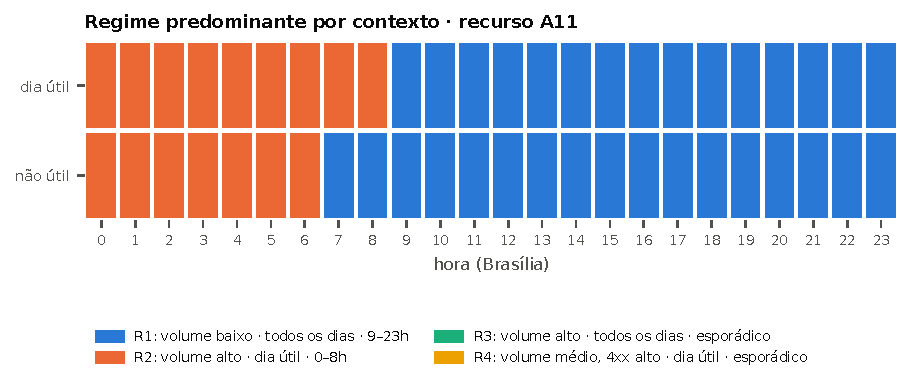
\includegraphics[width=0.85\textwidth]{figuras/fig_regimes_contexto.pdf}
  \caption{Regime predominante (k-means com os indicadores) por tipo de dia e hora no recurso A11.}
  \label{fig:regimes}
\end{figure*}

\begin{table*}[t]
  \caption{Resumo por recurso: participação no volume, clientes, transações medianas por 15~min, regimes e resultados no registro (faixa de 15~min, histórico de 3 meses).}
  \label{tab:recursos}
  \small
  \begin{tabular}{lrrrrrrrrr}
    \toprule
    Recurso & Vol. (\%) & Clientes & Trans./15 min & Regimes ($k$) & Silhouette & Sensib. & Sensib. média/alta & Especif. & Acurácia indicador \\
    \midrule
    A01 & 27,6 & 36    & 85.335 & 2 & 0,75 & 0,72 & 0,79 & 0,96 & 0,99 \\
    A02 & 26,0 & 45    & 67.001 & 2 & 0,66 & 0,66 & 0,75 & 0,97 & 0,99 \\
    A03 & 13,4 & 46    & 42.997 & 2 & 0,49 & 0,85 & 0,95 & 0,98 & 0,98 \\
    A04 & 11,1 & 45    & 34.148 & 2 & 0,69 & 0,87 & 0,92 & 0,99 & 0,99 \\
    A05 & 5,5  & 43    & 1.906  & 6 & 0,49 & 0,57 & 0,62 & 0,95 & 0,94 \\
    A06 & 5,3  & 21    & 14.840 & 6 & 0,57 & 0,26 & 0,27 & 1,00 & 1,00 \\
    A07 & 4,4  & 29    & 11.647 & 2 & 0,70 & 0,64 & 0,72 & 0,99 & 1,00 \\
    A08 & 1,5  & 5.390 & 3.999  & 2 & 0,47 & 0,39 & 0,47 & 0,93 & 0,95 \\
    A09 & 1,5  & 35    & 1.617  & 5 & 0,41 & 0,74 & 0,84 & 0,96 & 0,98 \\
    A10 & 1,1  & 37    & 1.240  & 5 & 0,39 & 0,58 & 0,63 & 0,96 & 0,96 \\
    A11 & 1,0  & 37    & 1.971  & 4 & 0,42 & 0,70 & 0,80 & 0,96 & 0,97 \\
    A12 & 1,0  & 4     & 2.843  & 2 & 0,43 & 0,63 & 0,75 & 0,99 & 0,99 \\
    A13 & 0,4  & 46    & 827    & 6 & 0,65 & 0,70 & 0,80 & 1,00 & 1,00 \\
    A14 & 0,2  & 37    & 453    & 5 & 0,42 & 0,48 & 0,50 & 0,98 & 0,99 \\
    \bottomrule
  \end{tabular}
\end{table*}

\subsection{Limites por indicador}
Os limites (Figura~\ref{fig:limites}) variam de 3 a 100 em $z$. Limites altos revelam indicadores com picos reais frequentes no histórico: erros 4xx em A06 (100), A05 (50), A08 (45) e A07 (42); volume em A05 (72), A13 (32) e A06 (29); e latência p95 em A02 (21). Nesses casos, só desvios grandes daquele indicador são marcados como \Residual. No histórico de junho a agosto, fora da amostra, 3,2\% das janelas de 1~h foram residuais, com latência (300 janelas), erros 4xx (290), volume (280) e erros 5xx (129) como indicadores responsáveis.

\begin{figure*}[t]
  \centering
  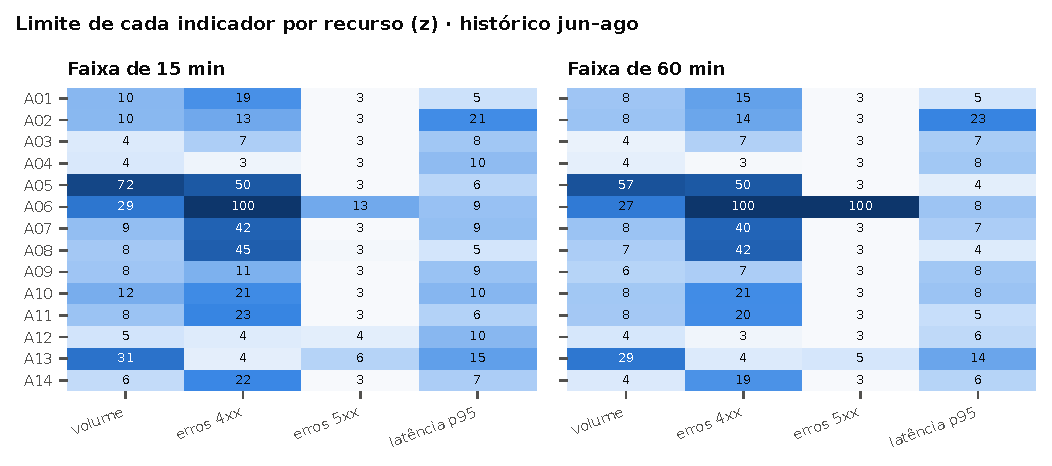
\includegraphics[width=0.85\textwidth]{figuras/fig_limites.pdf}
  \caption{Limite de cada indicador por recurso ($z$, percentil 99 fora da amostra, mínimo 3), para períodos de 15 e de 60~min; histórico de junho a agosto.}
  \label{fig:limites}
\end{figure*}

\subsection{Estado no instante do registro (RQ1)}
A Tabela~\ref{tab:metodos} e a Figura~\ref{fig:metodos} resumem a decisão. Com a faixa de 15~min, o perfil contextual classificou corretamente 97,3\% dos controles como \Normal e sinalizou como \Residual 63,0\% dos incidentes (70,6\% nas intensidades média e alta). Nos acertos de estado, ele supera o z-score global nas faixas de 15 e 30~min (McNemar: $p=0{,}009$ e $p=0{,}046$) e empata com a semana anterior em todas as faixas ($p\geq0{,}48$).

\begin{table*}[t]
  \caption{Estado no registro por método e faixa anterior ao registro, em \% (IC de Wilson a 95\% entre colchetes). Histórico de 3 meses; 4.411 incidentes e 4.480 controles.}
  \label{tab:metodos}
  \small
  \begin{tabular}{llccc}
    \toprule
    Método & Faixa $L$ & Sensibilidade & Sensibilidade (média/alta) & Especificidade \\
    \midrule
    \textbf{Perfil contextual (proposto)} & 15 min & \textbf{63,0} [61,6; 64,4] & \textbf{70,6} [68,8; 72,2] & 97,3 [96,7; 97,7] \\
     & 30 min & 60,3 [58,8; 61,7] & 68,3 [66,5; 70,0] & 97,2 [96,6; 97,6] \\
     & 60 min & 56,4 [55,0; 57,9] & 64,9 [63,1; 66,7] & 96,9 [96,3; 97,4] \\
    \midrule
    z-score global & 15 min & 61,0 [59,6; 62,4] & 68,8 [67,0; 70,5] & 98,0 [97,6; 98,4] \\
     & 30 min & 58,3 [56,8; 59,7] & 66,3 [64,5; 68,0] & 98,2 [97,7; 98,5] \\
     & 60 min & 54,5 [53,0; 55,9] & 62,5 [60,7; 64,3] & 98,4 [98,0; 98,7] \\
    \midrule
    Semana anterior & 15 min & 62,0 [60,6; 63,4] & 70,4 [68,6; 72,1] & 98,2 [97,8; 98,6] \\
     & 30 min & 59,6 [58,1; 61,0] & 68,3 [66,6; 70,1] & 98,2 [97,8; 98,6] \\
     & 60 min & 55,3 [53,8; 56,8] & 64,1 [62,3; 65,9] & 98,3 [97,9; 98,6] \\
    \bottomrule
  \end{tabular}
\end{table*}

\begin{figure*}[t]
  \centering
  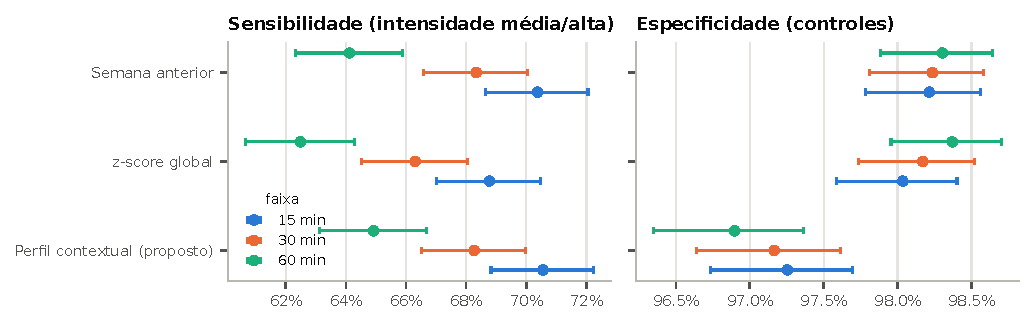
\includegraphics[width=0.85\textwidth]{figuras/fig_metodos.pdf}
  \caption{Sensibilidade (intensidades média e alta) e especificidade por método e faixa, com IC de Wilson a 95\%.}
  \label{fig:metodos}
\end{figure*}

\paragraph{Ponto de operação.} O limite de cada indicador é o seu percentil 99 no histórico (multiplicador $c=1$), ponto escolhido em versão anterior do estudo porque a consulta só é feita quando já existe um incidente aberto. A Figura~\ref{fig:curva} mostra também os pontos com 1\% e 2\% de alarmes no histórico. Nesses pontos mais conservadores, o z-score global detecta um pouco mais que o perfil contextual; no ponto adotado, o perfil contextual detecta mais, com 0,7 a 0,9 ponto a mais de falsos \Residual.

\begin{figure}[t]
  \centering
  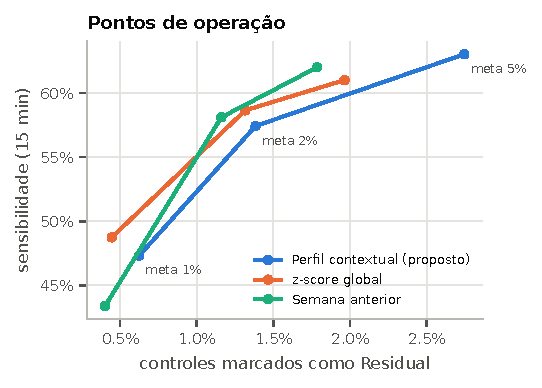
\includegraphics[width=0.85\columnwidth]{figuras/fig_curva_operacao.pdf}
  \caption{Sensibilidade contra controles marcados como \Residual (faixa de 15~min), para metas de 1\%, 2\% e 5\% de alarmes no histórico.}
  \label{fig:curva}
\end{figure}

\paragraph{Por motivo.} A sensibilidade depende do motivo (Figura~\ref{fig:sensmotivo}). Erros de sistema generalizados são detectados em 72\% a 99\% dos casos, conforme a intensidade, e erros 5xx de um consumidor em 74\% a 84\%. Erros de negócio têm detecção de 17\% a 66\% (generalizados) e de 36\% a 62\% (um consumidor). A latência vai de 13\% ($\times$1,5) a 72\% ($\times$4) e chega a \textbf{90\%} [86; 93] na degradação de 10 vezes.

\begin{figure}[t]
  \centering
  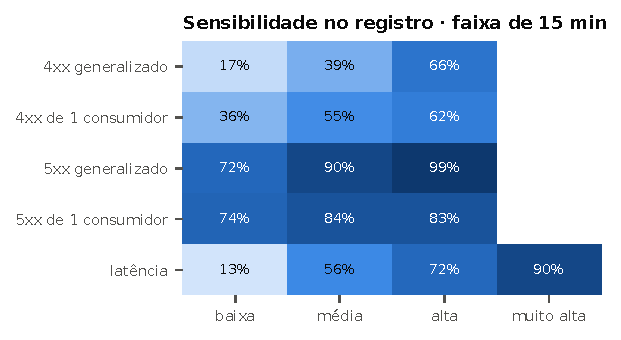
\includegraphics[width=0.9\columnwidth]{figuras/fig_sens_motivo.pdf}
  \caption{Sensibilidade no registro (faixa de 15~min) por motivo e intensidade.}
  \label{fig:sensmotivo}
\end{figure}

\paragraph{Por recurso e ao longo do teste.} Por recurso (Tabela~\ref{tab:recursos}), a sensibilidade vai de 26\% (A06, com limites de 4xx e 5xx muito altos e 23\% dos minutos sem dados) a 87\% (A04). Os quatro maiores recursos (A01 a A04) ficam entre 66\% e 87\%. O resultado é estável ao longo de setembro: 63,3\%, 60,6\% e 65,3\% de sensibilidade nas três semanas, com especificidade entre 95,5\% e 98,6\%.

\subsection{Tamanho da faixa e atraso do registro (RQ3)}
A faixa mais curta é a melhor quando o incidente é registrado logo após o início da degradação (Figura~\ref{fig:atraso}): com atraso de 15~min, a sensibilidade (intensidades média e alta) é de 74\% com a faixa de 15~min, contra 51\% com a de 60~min, que mistura minutos normais e degradados. Com atraso de 60 ou 120~min, a faixa de 60~min fica ligeiramente melhor (71--73\% contra 69--70\%). Na média, a faixa de 15~min é a melhor.

\begin{figure}[t]
  \centering
  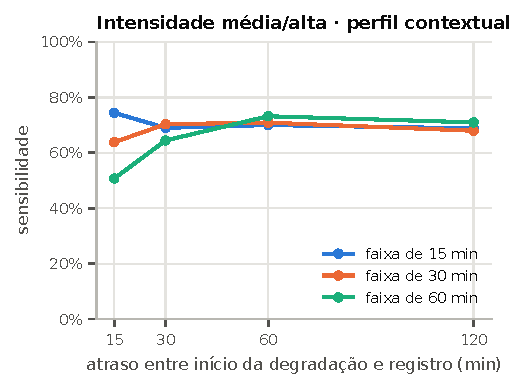
\includegraphics[width=0.85\columnwidth]{figuras/fig_sens_atraso.pdf}
  \caption{Sensibilidade (intensidades média e alta) por atraso entre o início da degradação e o registro, para cada tamanho de faixa.}
  \label{fig:atraso}
\end{figure}

\subsection{Histórico de 3 meses $\times$ 1 mês (RQ4)}
O histórico mais longo \emph{não} melhorou o resultado (Tabela~\ref{tab:historico}, Figura~\ref{fig:historico}). Com 1 mês, a sensibilidade subiu de 63,0\% para 67,0\% e a especificidade caiu de 97,3\% para 96,6\%; nos acertos de estado, o histórico de 1 mês foi melhor em todas as faixas (McNemar: $p<10^{-7}$). Os limites refletem a diferença: com 3 meses, o limite de erros 4xx fica, na mediana, 32\% maior, e chega a ser 14 vezes maior no A07 e 6 vezes maior no A01, recursos cuja taxa de 4xx caiu de junho para agosto.

\begin{table}[t]
  \caption{Histórico de 3 meses $\times$ 1 mês (proposto, faixa de 15~min, em \%; m/a = intensidades média e alta).}
  \label{tab:historico}
  \small
  \begin{tabular}{lcccc}
    \toprule
    Histórico & Sensib. & Sensib. m/a & Especif. & Acur. indicador \\
    \midrule
    3 meses & 63,0 & 70,6 & 97,3 & 98,2 \\
    1 mês & 67,0 & 72,9 & 96,6 & 98,5 \\
    \bottomrule
  \end{tabular}
\end{table}

\begin{figure}[t]
  \centering
  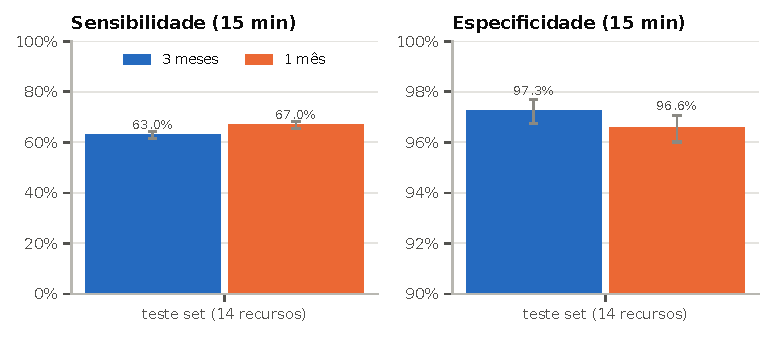
\includegraphics[width=0.9\columnwidth]{figuras/fig_historico.pdf}
  \caption{Sensibilidade e especificidade (faixa de 15~min) por histórico, com IC de Wilson a 95\%.}
  \label{fig:historico}
\end{figure}

\subsection{Indicador responsável e início (RQ2)}
Quando o recurso é sinalizado como \Residual, o indicador apontado é o do motivo injetado em 98,2\% dos casos [97,6; 98,6] (Figura~\ref{fig:confusao}): 99,3\% para 5xx generalizado, 98,6\% para 5xx de um consumidor e para latência, e 96--97\% para 4xx.

\begin{figure}[t]
  \centering
  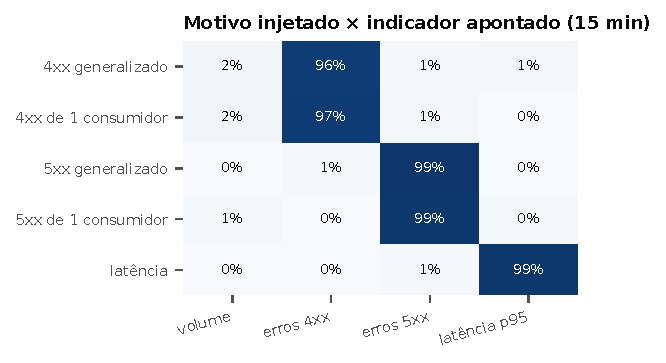
\includegraphics[width=0.85\columnwidth]{figuras/fig_confusao_indicador.pdf}
  \caption{Motivo injetado contra indicador apontado (faixa de 15~min, casos detectados).}
  \label{fig:confusao}
\end{figure}

A expansão retroativa (Figura~\ref{fig:expansao}) colocou o início real dentro da zona estimada em 94,8\% dos casos detectados [93,9; 95,6]: 98\% quando a degradação começou 15 ou 30~min antes do registro, 94\% com 60~min e 89\% com 120~min (Figura~\ref{fig:inicio}). Os erros são quase sempre subestimações: uma faixa intermediária sai \Normal, a busca para cedo e o início é estimado mais perto do registro do que de fato ocorreu.

\begin{figure*}[t]
  \centering
  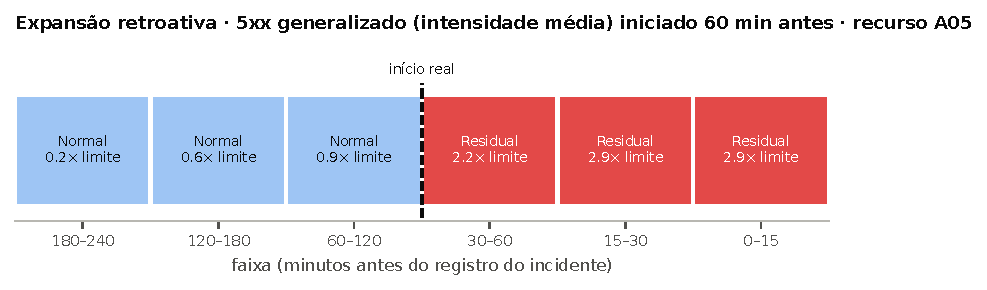
\includegraphics[width=0.85\textwidth]{figuras/fig_expansao_exemplo.pdf}
  \caption{Expansão retroativa em um cenário de 5xx generalizado iniciado 60~min antes do registro (A05): as três faixas mais recentes são residuais e a de 60--120~min é normal, e o início é estimado entre 30 e 120~min antes.}
  \label{fig:expansao}
\end{figure*}

\begin{figure}[t]
  \centering
  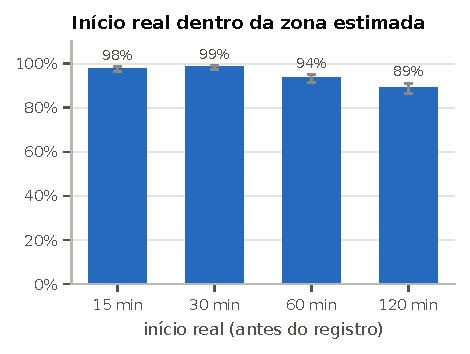
\includegraphics[width=0.8\columnwidth]{figuras/fig_inicio.pdf}
  \caption{Início real dentro da zona estimada, por atraso (IC de Wilson a 95\%).}
  \label{fig:inicio}
\end{figure}

\paragraph{Abrangência (complementar).} Entre os erros 4xx e 5xx detectados com o indicador correto, a abrangência foi classificada corretamente em 71,6\% [69,6; 73,4]. Os erros generalizados são reconhecidos como tais em 77--85\% dos casos; os de um consumidor, em 58\% (4xx) e 63\% (5xx). Uma parte relevante (14--26\%) fica indeterminada, porque nesses recursos há períodos de 15~min com menos de três clientes ativos.

\subsection{Saída para o agente e evento real}
A consulta produz um documento estruturado. A Figura~\ref{fig:json} mostra, resumida, a saída do cenário da Figura~\ref{fig:expansao}.

\begin{figure}[t]
\begin{Verbatim}[fontsize=\scriptsize,frame=single]
{"recurso": "A05", "registro_incidente": "2026-09-19 12:28",
 "contexto": {"tipo_dia": "não útil", "hora": "12h"},
 "estado": "Residual", "indicador_impactado": "erros 5xx",
 "evidencias": [{"indicador": "erros 5xx", "observado": "8.7%",
    "faixa_normal_p5_p95": ["0.0%", "0.0%"], "vezes_o_limite": 2.91}],
 "inicio_estimado": "entre 30 e 120 min antes do registro",
 "abrangencia": {"classificacao": "generalizado",
    "clientes_ativos": 4, "clientes_com_erro": 3},
 "motivo_estatistico": "O recurso A05 está fora do regime normal
   esperado para não útil às 12h. Indicador impactado: erros 5xx
   — 8.7% nos 15 min anteriores ao registro (faixa normal 0.0% a
   0.0%), 2.91× o limite do recurso. O desvio começou entre 30 e
   120 min antes do registro. Os erros aparecem em 3 de 4
   consumidores ativos."}
\end{Verbatim}
\caption{Saída da consulta para o agente (resumida).}
\label{fig:json}
\end{figure}

Nos dados reais, sem injeção, a primeira consulta de controle marcada como \Residual foi a do A12 às 22h46 de 11/09: latência p95 de 456~ms nos 15~min anteriores, com faixa normal de 123 a 149~ms para aquele contexto (1,77 vez o limite), e início estimado entre 0 e 30~min antes. É um candidato a degradação real de latência, a confirmar com a operação.

\subsection{Critérios de sucesso}
Os cinco critérios definidos antes da modelagem foram atendidos (Tabela~\ref{tab:criterios}), a sensibilidade por margem estreita.

\begin{table}[t]
  \caption{Critérios de sucesso (faixa de 15~min, histórico de 3 meses).}
  \label{tab:criterios}
  \small
  \begin{tabular}{p{0.5\columnwidth}p{0.22\columnwidth}c}
    \toprule
    Critério & Resultado & Atendido \\
    \midrule
    Controles com saída \Normal $\geq$ 95\% & 97,3\% & sim \\
    Sensibilidade (média/alta) $\geq$ 70\% & 70,6\% & sim \\
    Acurácia do indicador $\geq$ 90\% & 98,2\% & sim \\
    Início real na zona estimada $\geq$ 70\% & 94,8\% & sim \\
    Sem perda significativa para os baselines & sem perda & sim \\
    \bottomrule
  \end{tabular}
\end{table}

%% =====================================================================
\section{Discussão}\label{sec:discussao}

\paragraph{RQ1: regimes e estado no registro.} Os AALs agregados mostram regimes claros e ligados ao contexto, sobretudo à hora: lotes na madrugada, horário comercial e padrões diferentes em dias não úteis. O perfil contextual decide o estado de cada recurso no momento do incidente com alta especificidade (97,3\%) e sensibilidade de 63\% (71\% para degradações médias e altas). Em relação ao z-score global, o ganho é pequeno mas significativo; em relação à semana anterior, há empate. Além da detecção, o contexto dá a \emph{explicação}: a faixa normal do contexto, o regime esperado e o limite de cada indicador permitem dizer ao operador ``8,7\% de 5xx ao meio-dia de um sábado, quando o normal é zero''. Para o operador, um resultado \Residual é informação forte (raramente aparece sem motivo, e vem com o indicador certo); um resultado \Normal indica que o recurso dificilmente é a origem, mas não descarta degradações sutis.

\paragraph{O efeito do volume.} Os resultados desta versão são bem melhores que os obtidos com recursos de menor volume em versões anteriores do estudo (sensibilidade de 39\% e 43\% nas intensidades média e alta). Com dezenas de milhares de transações por 15~min, as taxas de erro e o p95 variam menos dentro de cada contexto, os limites ficam mais estreitos e as degradações aparecem com mais clareza. Os quatro maiores recursos (A01 a A04) têm sensibilidade de 66\% a 87\%. Isso sugere que o método é mais útil justamente nas APIs de maior volume, que tendem a ser as mais críticas.

\paragraph{RQ2: indicador e início.} O ponto mais forte do método é a qualidade da informação quando ela é emitida: o indicador responsável é apontado corretamente em 98\% dos casos, e o início é localizado na zona certa em 95\%. A expansão retroativa é simples de explicar (``olhar para trás até encontrar um período normal'') e dá ao operador uma resposta útil em faixas de 15~min a 1~h, que é a escala em que incidentes costumam ser abertos.

\paragraph{RQ3: tamanho da faixa.} A faixa de 15~min é a melhor escolha como decisão principal, porque o incidente costuma ser aberto pouco depois do início da degradação. Faixas maiores só compensam quando a degradação já dura uma hora ou mais. Na prática, a faixa curta decide o estado e a expansão retroativa dá o horizonte.

\paragraph{RQ4: quanto histórico.} Pela segunda vez no estudo, e agora com outro conjunto de recursos, mais histórico não significou um perfil melhor. As APIs mudam de patamar ao longo dos meses, e um histórico de três meses inclui comportamentos que já não valem (por exemplo, taxas de erros de negócio que depois caíram), o que alarga os limites. Para a implantação, isso favorece o \emph{retreino frequente com o histórico recente} (por exemplo, mensal com o último mês) em vez de acumular meses.

\paragraph{Onde o método detecta pouco.} Erros de negócio de baixa intensidade (5\% de 4xx generalizado) raramente são detectados, porque vários recursos têm taxas de 4xx naturais altas e variáveis. Recursos com picos reais frequentes (4xx em A05, A06, A07 e A08) recebem limites altos e só mostram desvios grandes; no A06, com limites de 4xx e 5xx muito altos e minutos sem dados, a sensibilidade foi de 26\%. Nesses casos, o próprio limite é uma informação útil: ele diz ao operador que aquele indicador já é instável no recurso.

%% =====================================================================
\section{Ameaças à validade}\label{sec:ameacas}

\paragraph{Falhas sintéticas.} O desempenho mede a capacidade de detectar \emph{os motivos injetados}. As intensidades variadas, os quatro atrasos e o grande número de cenários reduzem, mas não eliminam, esse viés.

\paragraph{Decisões tomadas ao longo do estudo.} O ponto de operação (limite no percentil 99), a intensidade de latência $\times$10 e a limitação dos indicadores aos percentis 1 e 99 no k-means foram definidos em versões anteriores do estudo, com outros recursos e períodos, e mantidos sem alteração nesta versão. O histórico principal (3 meses) foi fixado antes de observar os resultados, e o resultado desfavorável a ele é relatado. O critério de sensibilidade foi atingido por margem estreita (70,6\% contra 70\%), e o seu intervalo de confiança (68,8\% a 72,2\%) inclui valores abaixo da meta.

\paragraph{Seleção dos recursos.} Foram usados apenas recursos com dados em todos os dias do período, o que favorece recursos estáveis e de alto volume. Os quatro descartados (21\% do volume) poderiam ter comportamento diferente. Dois recursos incluídos (A05 e A06) têm minutos sem dados, e 69 incidentes simulados caíram nesses intervalos e foram excluídos.

\paragraph{Controles e anomalias reais.} As consultas de controle usam dados reais sem injeção, que podem conter anomalias reais (como a do A12), contadas como falso \Residual. A especificidade é, portanto, uma estimativa conservadora.

\paragraph{Latência aproximada.} O p95 é calculado sobre as médias por minuto e por cliente, e não sobre requisições; a cauda real tende a ser maior. Uma latência 10 vezes maior poderia, na prática, esbarrar no \emph{timeout} do gateway e virar erro 504, o que a injeção não simula.

\paragraph{Período e generalização.} O teste cobre 20 dias de setembro, com um feriado (07/09); os feriados considerados foram 04/06 (Corpus Christi, tratado como não útil) e 07/09. Os resultados vêm de uma organização e de 14 recursos. A base não pode ser compartilhada; o código dos notebooks é independente dos dados.

%% =====================================================================
\section{Considerações finais}\label{sec:conclusao}

Este trabalho mostrou que Access Logs agregados por minuto, sem \emph{traces} nem logs de aplicação, permitem caracterizar os regimes normais de cada recurso de API e informar, no instante em que um incidente é aberto, se o recurso está em regime normal e, se não, qual indicador foi impactado (erros de negócio, erros de sistema ou latência) e desde quando. O método usa técnicas simples (mediana, MAD, percentis, validação cruzada e uma busca retroativa), não exige rótulos e produz uma explicação que um agente ou operador pode usar diretamente.

Em 14 recursos de alto volume, a informação foi confiável e útil: 97,3\% de especificidade, 63\% de sensibilidade (71\% nas degradações médias e altas; até 99\% para erros de sistema e 90\% para latência de 10 vezes), 98,2\% de acerto no indicador e 94,8\% de acerto na zona de início. Os cinco critérios de sucesso foram atendidos. O ponto fraco são os erros de negócio de baixa intensidade em recursos com muitos 4xx naturais. O histórico recente (1 mês) mostrou-se melhor que o longo (3 meses), o que recomenda retreino frequente.

Como trabalhos futuros, destacam-se: (i) validar o método com incidentes reais, começando pelo evento de latência observado no A12, e com a avaliação de operadores; (ii) adotar o histórico de 1 mês com retreino mensal e avaliar janelas deslizantes ponderadas; (iii) melhorar a sensibilidade a erros de negócio e à latência com percentis por requisição; (iv) avaliar recursos de menor volume e outras APIs; e (v) integrar a consulta como ferramenta de um agente de apoio a incidentes.

\bibliographystyle{ACM-Reference-Format}
\bibliography{referencias}

\end{document}
